%=============================================================================
\documentclass[10pt,a4paper]{article}
%
%
%
\usepackage{graphicx}
\usepackage{hyperref}
\usepackage{verbatim}
\usepackage{fix-cm}
\usepackage{lineno}
\usepackage{fancyhdr}
%
\usepackage{amsmath}
%
\oddsidemargin  0.1 in
\evensidemargin 0.1 in
%
%
\newlength{\backindent}\setlength{\backindent}{2cm}
\textwidth 5.375 in % Width of text line.
\advance\textheight by1.4cm
\advance\voffset by-1.4cm
\advance\textwidth by\backindent
%
%
% === Fancy headers setup  ===============================
%
\setlength{\headheight}{15.2pt}
\pagestyle{fancyplain} {
\fancyhead[L]{
\includegraphics[height=10mm]{DD4hep-AIDA-logo.png}\vspace{-0.3cm}}
\fancyhead[C]{}
\fancyhead[R]{\sffamily{\underline{\hspace{6cm}Advanced European Infrastructures for Detectors at Accelerators}}}
\fancyfoot[L]{}
\fancyfoot[C]{\sffamily{User Manual}}
\fancyfoot[R]{\sffamily{\thepage}}
}
%
%
\newcommand{\tw}[1]{${\tt{#1}}$}
\newcommand{\tts}[1]{{\tt\small{#1}}}
\newcommand{\bold}[1]{{\bf{#1}}}
%
%
\newcommand{\DDE}{{$\tt{DDEve}$\space}}
\newcommand{\DDhep}{{$\tt{DD4hep}$\space}}
\newcommand{\DDH}{{$\tt{DD4hep}$\space}}
\newcommand{\DDG}{{\tt{DDG4}\space}}
\newcommand{\DDA}{{\tt{DDAlign}\space}}
\newcommand{\DDR}{{\tt{DDRec}\space}}
%
%
\newcommand{\docline}[2]{\vspace{0.1cm}{\bf{#1}} & \parbox{14.5cm}{#2}\\}
%
% === Specialization of the lineno package
%
\renewcommand{\linenumberfont} {\normalfont\small\sffamily}
\renewcommand{\makeLineNumber} {\makeLineNumberLeft}
\renewcommand{\linenumbersep} {2pt}
%
% === Set font to code section with line numbers
%
\newenvironment{code}{\par\vspace{0.01cm}\small\linenumbers\verbatim\setcounter{linenumber}{1}}{\endverbatim\nolinenumbers\vspace{-0.02cm}}%
%
% === Set font to code section with line numbers
%
\newenvironment{unnumberedcode}{\par\vspace{-0.1cm}\small\verbatim\setcounter{linenumber}{1}}%
{\endverbatim\vspace{-0.2cm}}
%
% === Command to insert http links to the DD4hep geomtery package
%
\newcommand{\detdesc}[2]
{
    \href{http://www.cern.ch/frankm/DD4hep/#1}{#2}
}
%
% === Command to insert http links to the ROOT geomtery package
%
\newcommand{\tgeo}[2]
{
    \href{http://root.cern.ch/root/html/#1.html}{#2}
}
\newcommand{\tgeoO}[3]
{
    \href{http://root.cern.ch/root/html/#1:#2}{#3}
}
%
% ===  Compactify the item list  =========================
%
\newcommand{\itemcompact}{\setlength{\itemsep}{1pt}\setlength{\parskip}{0pt}\setlength{\parsep}{0pt}}
%
%
% ===  Title page command  ===============================
%
%
\newcommand{\basictitle}[2]{
%
\pagestyle{empty}
%

\includegraphics[height=25mm] {DD4hep-AIDA-logo.png}

\vspace{0.02cm}

{\sffamily{\underline{\hspace{6cm}Advanced European Infrastructures for Detectors at Accelerators}}}

\vspace{2cm}

\begin{center}
{\fontsize{72}{32}\selectfont{\bfseries{#1}}}

\vspace{3cm}
{\Huge\bf{#2}}
\vspace{3cm}

\end{center}
}


\newcommand{\mytitle}[3]{
\begin{titlepage}
\basictitle{#1}{#2}
\begin{center}
{#3}

%%M.Frank %%\textsuperscript{1}
%%%F.Gaede\textsuperscript{2},
%%%C.Grefe\textsuperscript{1}
%%\vspace{1cm}
%%\textsuperscript{1}
%%{CERN, 1211 Geneva 23, Switzerland}
%%%{\textsuperscript{2} {Desy, 22607 Hamburg, Germany}
\end{center}
\end{titlepage}
}

%
\pagestyle{fancyplain}{\fancyfoot[C]{\sffamily{DRAFT -- DDEve User Manual -- DRAFT}}}
%
\begin{document}   
%
\mytitle{
DDEve
}{
An Event Display for \\
\vspace{0.5cm}
DD4hep Geometries \\
\vspace{2.5cm}
-- DRAFT -- \\
}
{M. Frank \\
{CERN, 1211 Geneva 23, Switzerland}}
%
%
%==  Abstract  ===============================================================
\pagestyle{plain}
\pagenumbering{Roman}
\setcounter{page}{1}
\begin{abstract}
%=============================================================================

\noindent
\normalsize
\DDE is a framework implementing a event display for detector geometries
implemented using DD4hep. \DDE hereby takes advantage of the TEve toolkit
naturally provided by the ROOT framework like the ROOT geometry toolkit
TGeo. 
\noindent
\DDE actively uses the collaboration between TEve and TGeo as well 
as the various object collaborations provided by the toolkits.
\DDE does in no way intend to hide any of the two toolkits, but 
rather provides facilities to construct various detector views 
in the most suitable manner using predefined configurations.
\end{abstract}

\vspace{8cm}

\begin{center}
{\large{\bf{
\begin{tabular} {| l | l | l |}
\hline
\multicolumn{3}{| c |}{} \\[0.2cm]
\multicolumn{3}{| c |}{Document History} \\[0.2cm]
\multicolumn{3}{| c |}{} \\[0.2cm]
\hline
                 &      &        \\
Document         &      &        \\
version          & Date & Author \\[0.2cm] \hline
                 &      &        \\
1.0              & 15/08/2014 & Markus Frank CERN/LHCb  \\
                 &      &        \\        \hline 
\end{tabular}
}}}
\end{center}

\clearpage
%
%
%==  TOC  ====================================================================
\tableofcontents
\clearpage
%
%
%=============================================================================
% Manual
%=============================================================================
\pagenumbering{arabic}
\setcounter{page}{1}

%=============================================================================
\section{Introduction}
\label{sec:ddeve-user-manual-introduction}
%=============================================================================
\noindent
Short usage description of \DDE.

\noindent
\DDE is a purely experimental package. It was developed to 
\begin{itemize}
\item visually debug developed detector geometries including partial views 
       using predefined displays.
\item compensate the frustration caused by the slow progress of subdetector 
       geometry implementers, which did not get up to speed and hence did not
       require any support from me.....
\end{itemize}
Since up to now \DDE is a hobby of mine, please do not expect a great deal 
of documentation and support.

%=============================================================================
\section{Running the CLICSiD Example}
\label{sec:ddeve-user-manual-introduction}
%=============================================================================
\noindent
DDEve is started using the root executable. In the following we describe 
how to start a display application of \DDE using the CLICSiD example.
\begin{unnumberedcode}
$> root.exe $DD4hepINSTALL/examples/DDEve/DDEve.C 
\end{unnumberedcode}
When the command is issued the following display shows up:
\begin{figure}[h]
  \begin{center}
    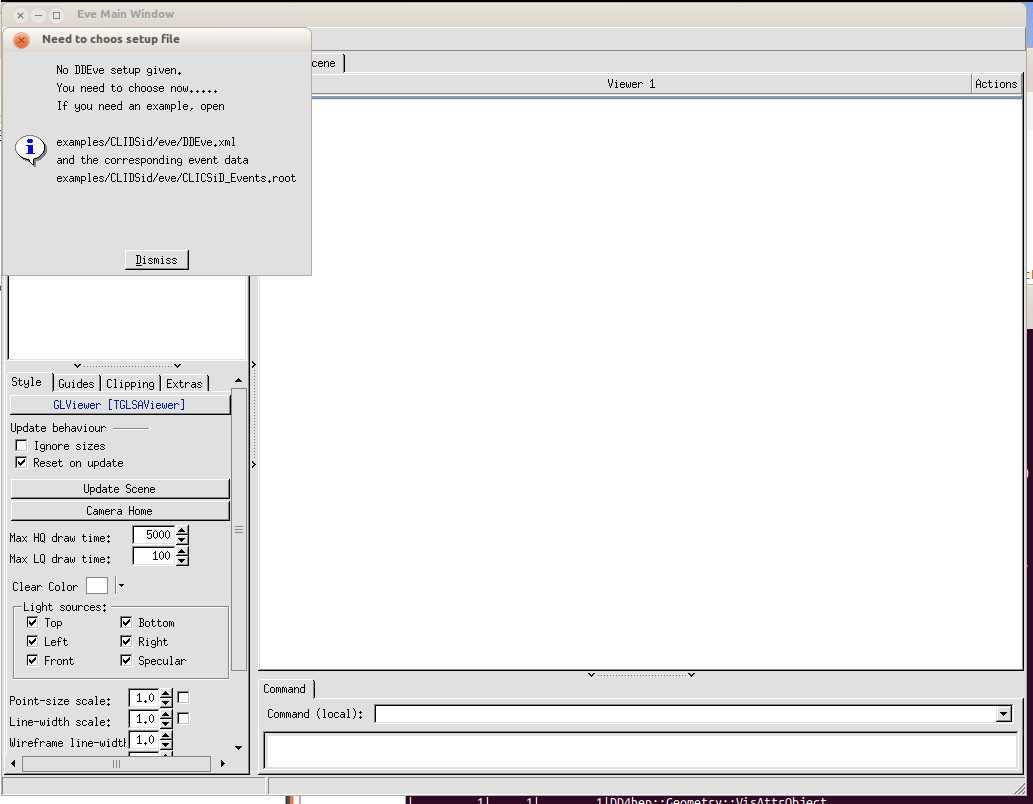
\includegraphics[height=90mm] {DDEve_1.png}
    \caption{The \DDE startup view.}
    \label{fig:DDEve_1.png}
  \end{center}
\end{figure}
\newpage
\noindent
Click on "Dismiss" then the file browser opens and you have to select 
a \DDE configuration file:
\begin{figure}[h]
  \begin{center}
    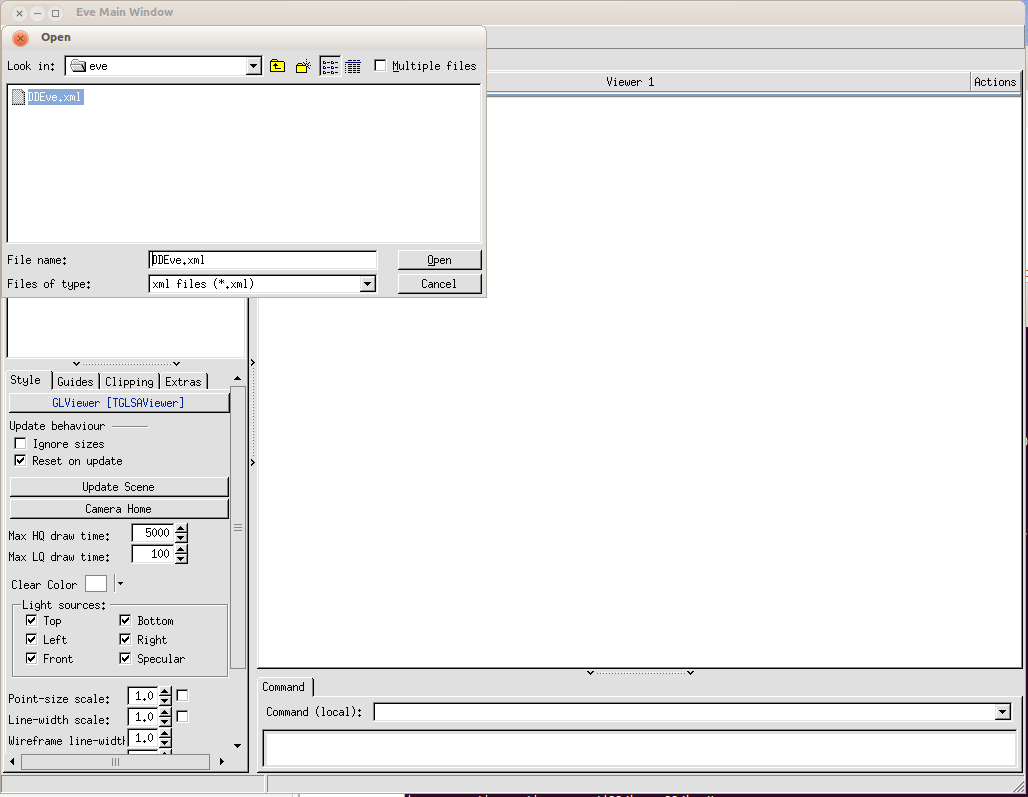
\includegraphics[height=120mm] {DDEve_2.png}
    \caption{The \DDE popup dialog to open the XML configuration file.}
    \label{fig:DDEve_2.png}
  \end{center}
\end{figure}

\noindent
Move to the directory \tts{\$DD4hepINSTALL/examples/CLIDSid/eve} and open the 
\DDE configuration file \tts{DDEve.xml}. The basic idea is that \DDE as an 
application is truely generic and that all subsequent behavior 


\newpage
\noindent
Next you should see the default pane with the instantiated CLICSiD detector:

\begin{figure}[t]
  \begin{center}
    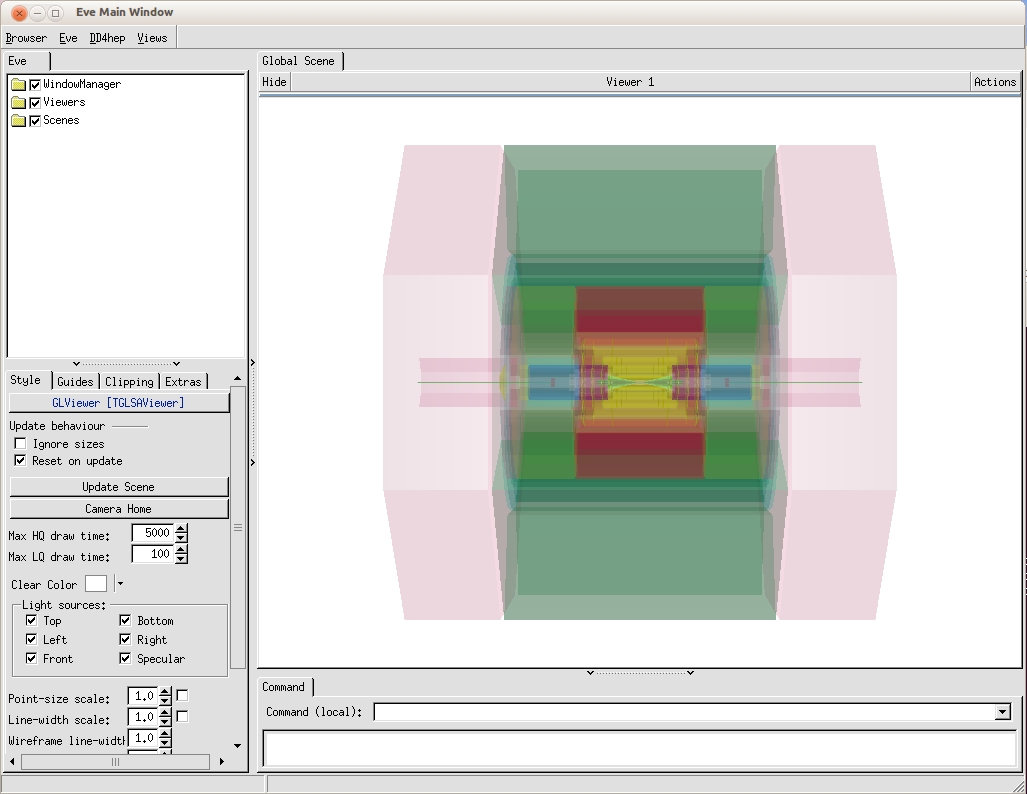
\includegraphics[height=120mm] {DDEve_3.png}
    \caption{The \DDE default view showing the loaded detector.}
    \label{fig:DDEve_3.png}
  \end{center}
\end{figure}

\newpage
\noindent
Then open from the \tts{"DD4hep"} menu the item \tts{"Open Event Data"}. Move again to the 
directory \tts{\$DD4hepINSTALL/examples/CLIDSid/eve} and open the sample file
\tts{CLICSiD\_Events.root} containing a sample of events being the output of 
a \DDG simulation step:

\begin{figure}[h]
  \begin{center}
    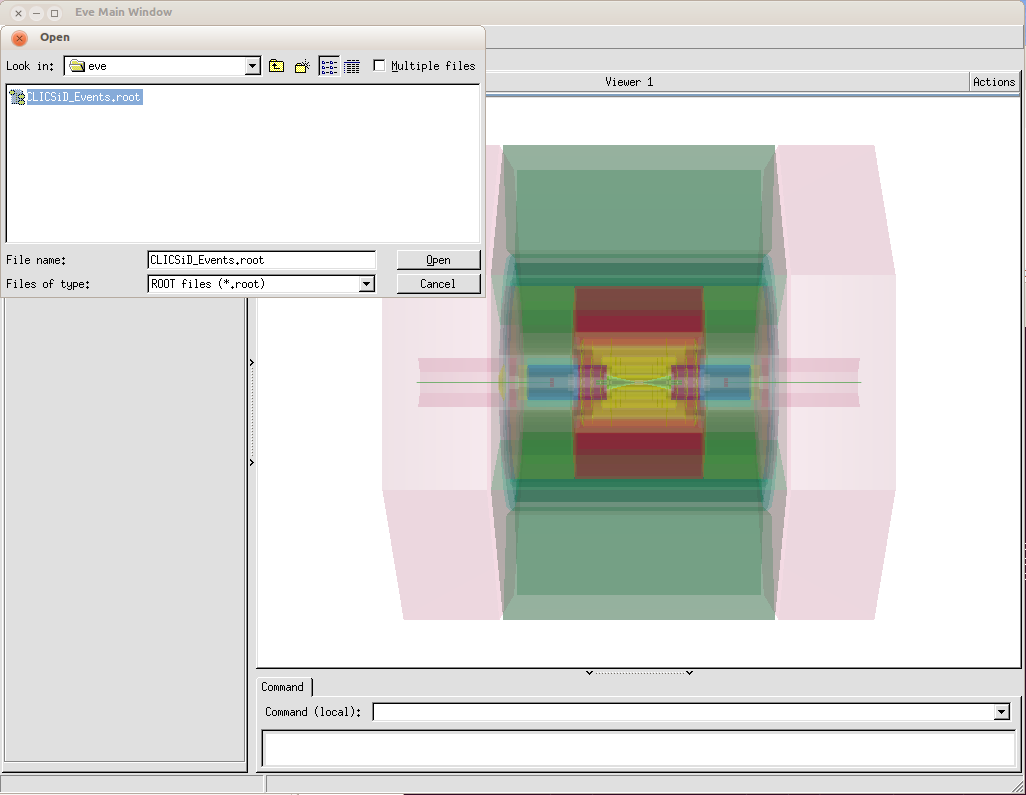
\includegraphics[height=130mm] {DDEve_4.png}
    \caption{The popup dialog to open event data files.}
    \label{fig:DDEve_4.png}
  \end{center}
\end{figure}
Using the \tts{"Views"} menu other predefined detector views may be used.

\newpage
\noindent 
The \tts{"Eve"} tab on the pane to the left allows to further customize the 
predefined views, the \tts{Evt I/O} tab to control which event should 
be displayed.

\begin{figure}[h]
  \begin{center}
    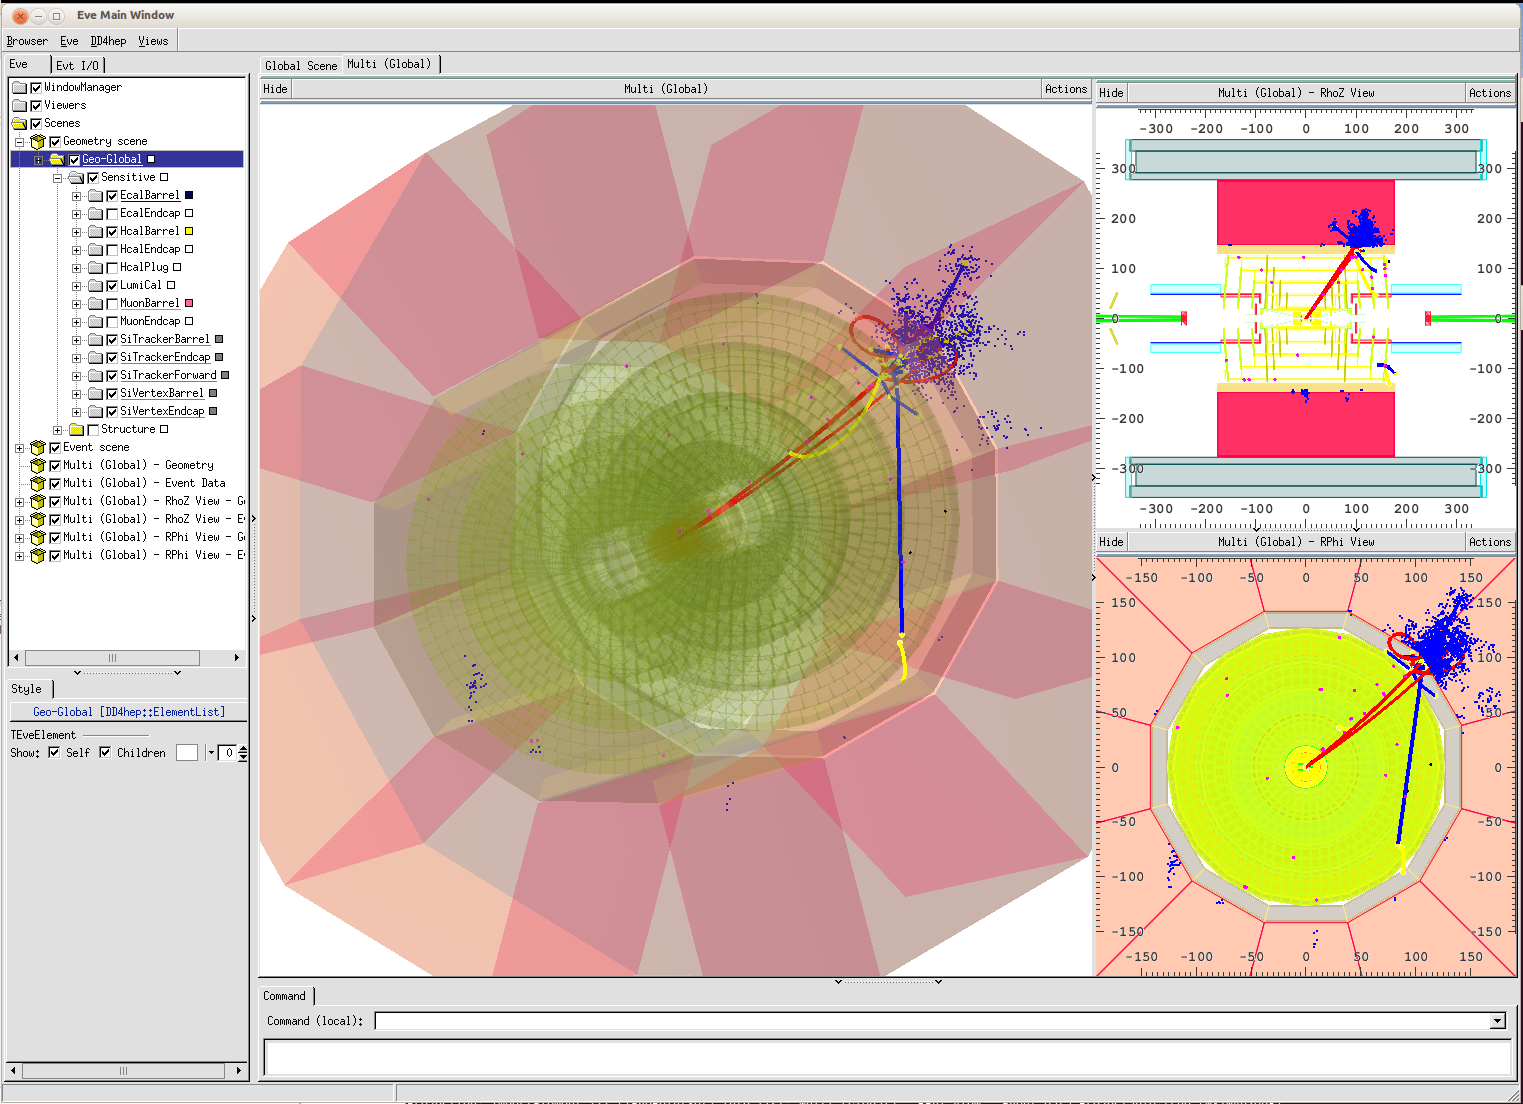
\includegraphics[height=130mm] {DDEve_5.png}
    \caption{An example of a customized view with sub-panes. Please proceed 
               to the XML configuration file how to create a predefined view.}
    \label{fig:DDEve_5}
  \end{center}
\end{figure}

\newpage
\noindent
\begin{figure}[h]
  \begin{center}
    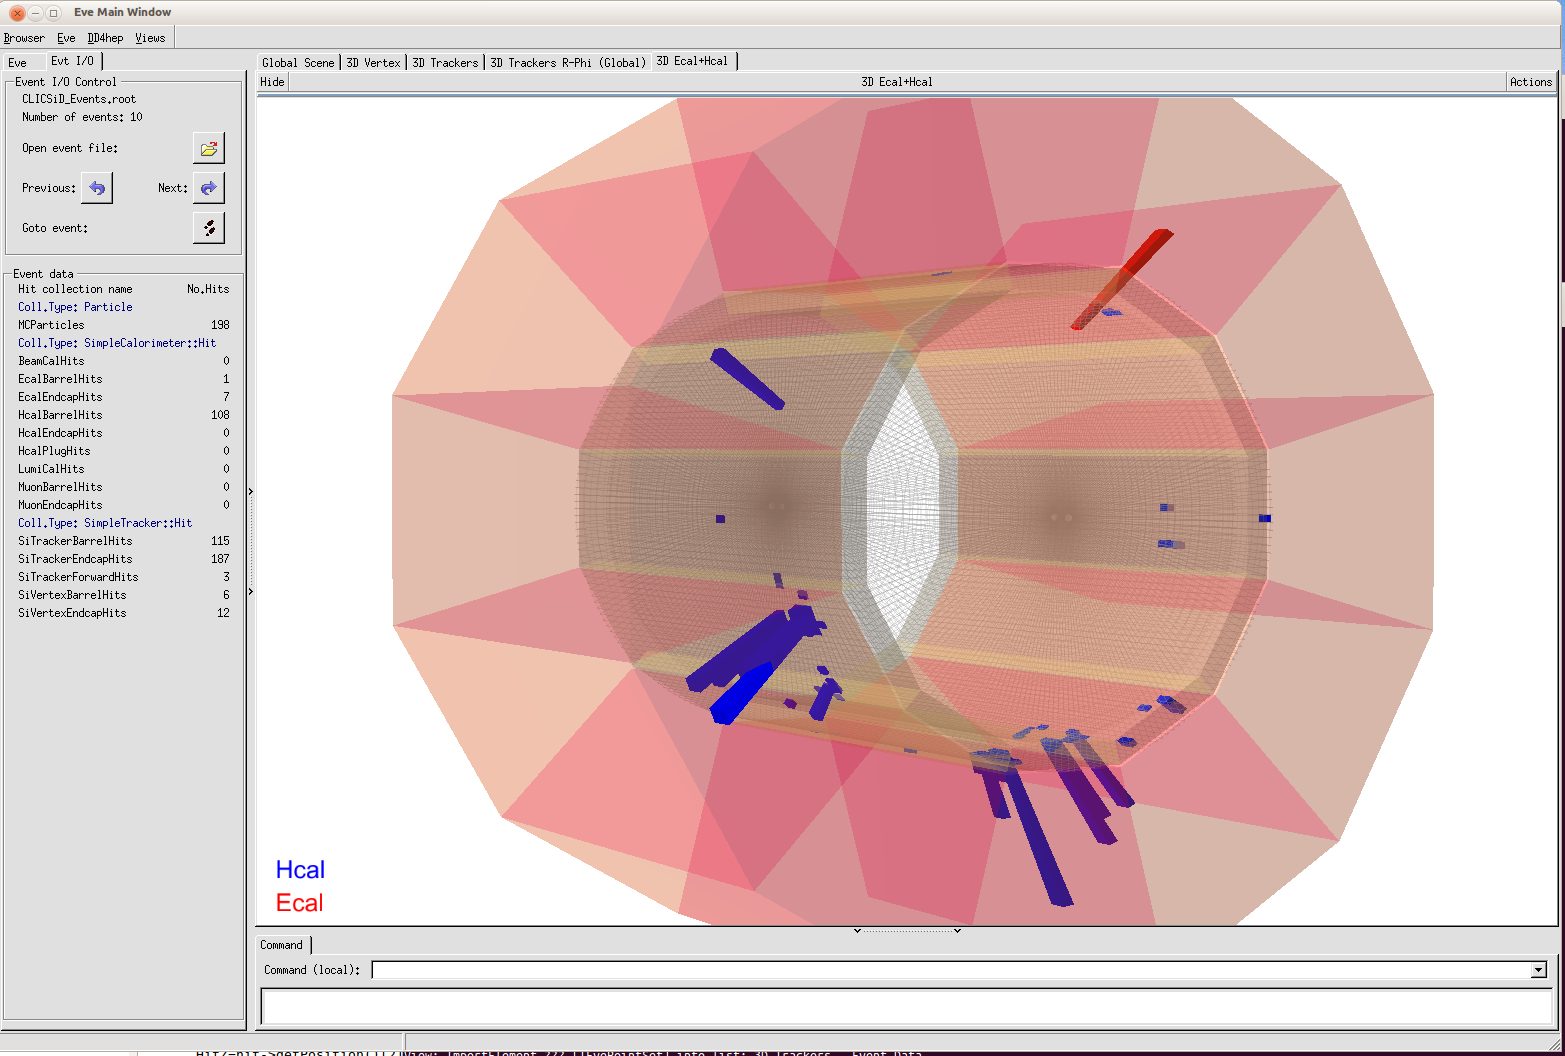
\includegraphics[height=130mm] {DDEve_7.png}
    \caption{Calorimetr energy deposits in the ECAL (red) and the HCAL(blue).}
    \label{fig:DDEve_5}
  \end{center}
\end{figure}

\newpage
\noindent
\begin{figure}[h]
  \begin{center}
    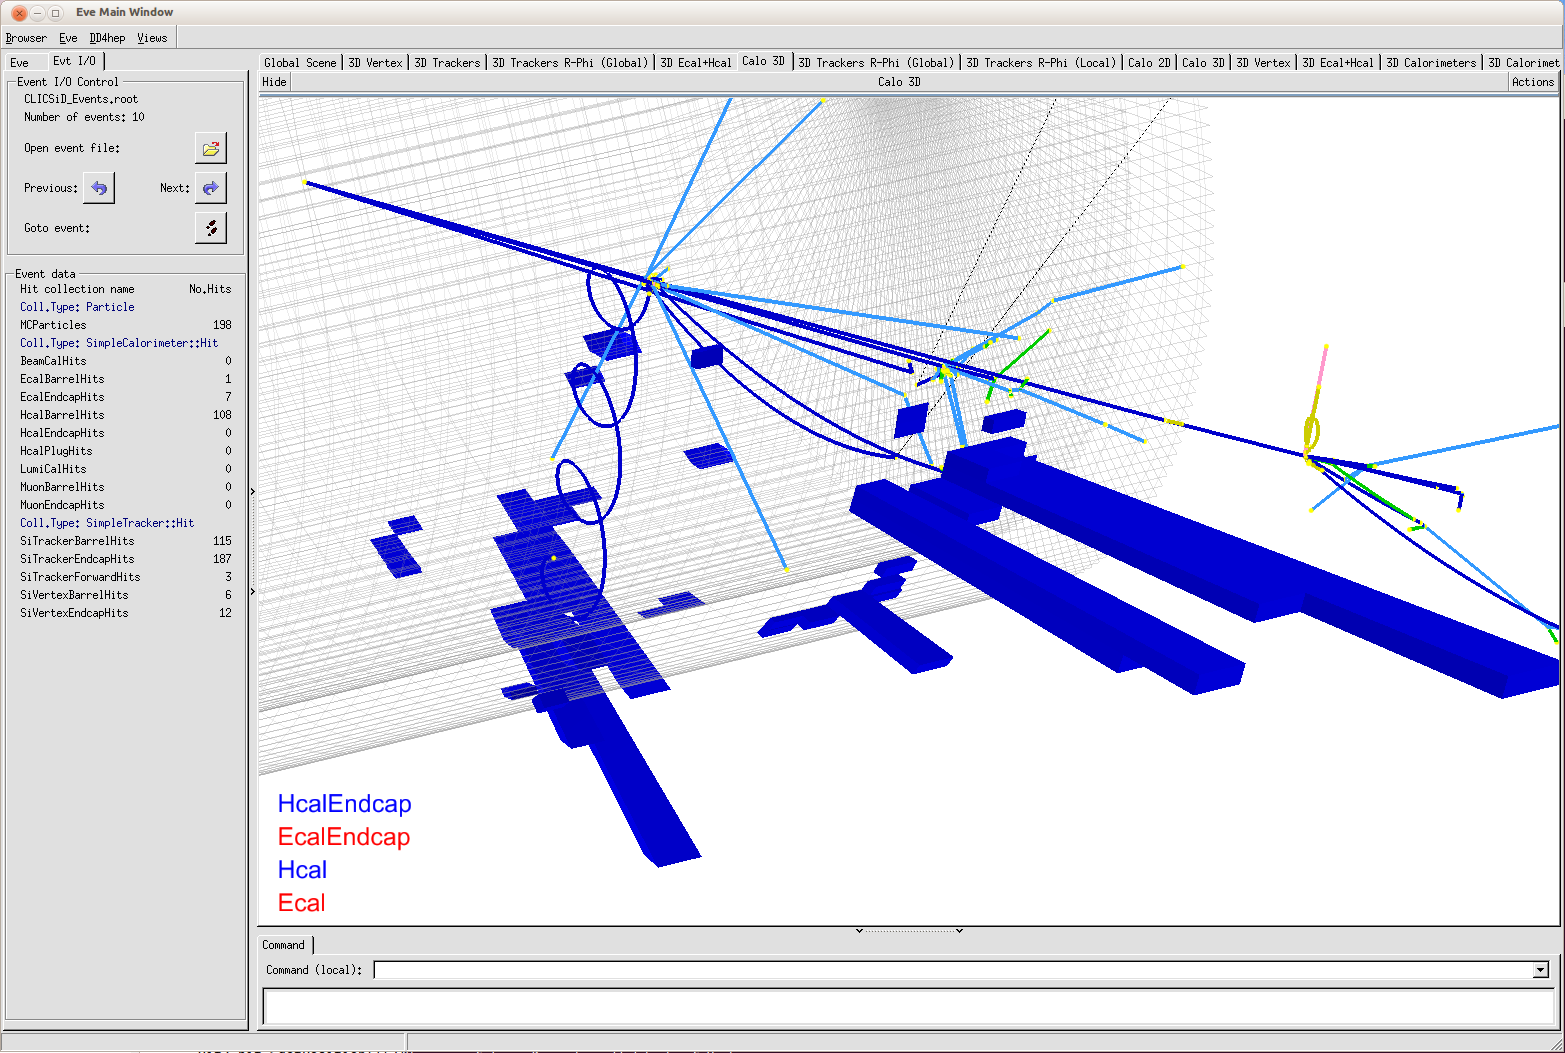
\includegraphics[height=130mm] {DDEve_8.png}
    \caption{HCAL calorimeter deposits together with Monte-Carlo tracks.}
    \label{fig:DDEve_5}
  \end{center}
\end{figure}


%=============================================================================
\section{View Configuration}
\label{sec:ddeve-user-manual-display-configuration}
%=============================================================================
\noindent
This part of the \DDE application is not really stable. to configure displays
other than for the \tts{CLICSiD} example, you have to use the trial and error 
approach. Starting from the \tts{CLICSiD} example is not too bad an approach.


%=============================================================================
\newpage
\begin{thebibliography}{9}
\bibitem{bib:DD4hep}  DD4Hep web page, http://aidasoft.web.cern.ch/DD4hep.

\bibitem{bib:LHCb} 		LHCb Collaboration, 
                "LHCb, the Large Hadron Collider beauty experiment, reoptimised detector 
				design and performance", CERN/LHCC 2003-030

\bibitem{bib:LHCb-geometry} S. Ponce et al., 
                "Detector Description Framework in LHCb", 
                International Conference on Computing in High Energy and Nuclear Physics  (CHEP 2003), 
                La Jolla, CA, 2003, proceedings. 

\bibitem{bib:ILD}  The ILD Concept Group, 
                   "The International Large Detector: Letter of Intent",\\
                   ISBN 978-3-935702-42-3, 2009.

\bibitem{bib:SiD}  H. Aihara, P. Burrows, M. Oreglia (Editors),
                   "SiD Letter of Intent",
                   arXiv:0911.0006, 2009.

\bibitem{bib:ROOT-tgeo} R.Brun, A.Gheata, M.Gheata, "The ROOT geometry package",\\
                    Nuclear Instruments and Methods {\bf{A}} 502 (2003) 676-680.

\bibitem{bib:ROOT} R.Brun et al., 
                   "Root - An object oriented data analysis framework",\\
                    Nuclear Instruments and Methods {\bf{A}} 389 (1997) 81-86.

\bibitem{bib:geant4}  S. Agostinelli et al., 
                   "Geant4 - A Simulation Toolkit", \\
                    Nuclear Instruments and Methods {\bf{A}} 506 (2003) 250-303.

\bibitem{bib:LCDD} T.Johnson et al., 
                   "LCGO - geometry description for ILC detectors", 
                   International Conference on Computing in High Energy and Nuclear Physics  (CHEP 2007), 
                   Victoria, BC, Canada, 2012, Proceedings.

\bibitem{bib:lcsim} N.Graf et al., 
                   "lcsim: An integrated detector simulation, 
                   reconstruction and analysis environment", 
                   International Conference on Computing in High Energy and Nuclear Physics (CHEP 2012),
                   New York, 2012, Proceedings.

\bibitem{bib:GDML} R. Chytracek et al.,
                   "Geometry Description Markup Language for Physics Simulation and Analysis
                   Applications",
                   IEEE Trans. Nucl. Sci., Vol. 53, Issue: 5, Part 2, 2892-2896,
                   http://gdml.web.cern.ch.

\end{thebibliography}
%=============================================================================
\end{document}
